\documentclass[conference,a4paper]{IEEEtran}
\usepackage{graphicx}
\usepackage{amsmath}
\usepackage{booktabs}
\usepackage{url}

\begin{document}

\title{Teaching an Agent to Beat the Dealer: Tabular Reinforcement Learning for Blackjack Strategy, Card Counting, and Bet Sizing}

\author{
\IEEEauthorblockN{Rafsan Bari Shafin}
\IEEEauthorblockA{Technical University of Applied Sciences W\"urzburg-Schweinfurt\\
Reasoning and Decision Making under Uncertainty --- Portfolio Exam 3\\
Summer 2026}
}

\maketitle

\begin{abstract}
This paper builds a Blackjack-playing agent using only tabular reinforcement
learning, written in plain Python with no external RL library anywhere in
the project. The agent is trained on four scenarios of growing difficulty:
basic strategy on a standard six-deck game; a full Hi-Lo card-counting
system with a learned bet-sizing policy; the same two setups replayed under
two different rule sets, to see how the rules push the learned strategy
around; and an attempt to improve the counting system so it earns more
money on average. Each trained policy is frozen and evaluated over two
million hands, giving a profit estimate with a 95\% confidence interval.
Along the way, the first version of the bet-sizing agent broke in a way
that turned out to be genuinely instructive: it learned to never change the
bet at all. Fixing that is as much a part of this paper as the final
results are. Monte Carlo control clearly beats Q-learning on this task. The
learned basic strategy matches Thorp's published tables on most states. The
two rule changes move the policy exactly where basic theory says they
should. And the repaired betting system turns a confidently losing counting
strategy into one that is statistically indistinguishable from break-even.
\end{abstract}

\section{Introduction}
Blackjack is a good place to study decision-making under uncertainty. It is
small enough to write down as a finite Markov Decision Process; Sutton and
Barto use it as one of their running examples \cite{suttonbarto}. At the
same time, it is the one casino game where a disciplined player can gain a
genuine mathematical edge over the house. Edward Thorp proved this and
popularized it with the Hi-Lo point-count system in \emph{Beat the Dealer}
\cite{thorp}. Both properties together make it a good testbed for tabular
reinforcement learning. The base game fits comfortably into a lookup table.
Adding card counting, however, turns the problem into something closer to a
partially observable process, since the composition of the remaining shoe
changes the odds from hand to hand and has to be folded into the state
somehow for a stationary policy to make sense at all.

This paper documents a from-scratch implementation built for that purpose.
No external reinforcement-learning framework is used anywhere in the code,
as the assignment requires. Four things were asked for: (1) recover basic
strategy purely by playing hands and updating value estimates, (2) learn a
complete point-count system together with a bet that reacts to the count,
(3) see what happens to both of the above under two different rule
variants, and (4) actually improve on the point-count system, not just
implement it again. We also try to answer, honestly and with numbers rather
than assertions, four questions the assignment asks directly: which
learning algorithm behaves better here and why; how big the resulting
state-action space actually is, and whether the resulting $Q$-values can be
trusted; why the two rule changes move the policy the way they do; and how
we know the profit numbers we report are not just noise.

One thing worth saying up front: this project did not work correctly on
the first try. The initial bet-sizing agent for the counting scenario
passed every basic sanity check we ran, and still converged to a policy
that never bet more than the table minimum. Once Scenario 4 added a sit-out
option, the same agent learned to sit out \emph{every single hand},
reporting a profit of exactly zero. Section~\ref{sec:betting} explains why,
because the failure is a useful example of what goes wrong when a
bandit-style estimator has to resolve a signal that is small compared to
its own sampling noise.

Section~\ref{sec:method} describes the simulator, the state representation,
and both learning algorithms, including the betting-agent story above.
Section~\ref{sec:experiments} gives the experimental setup, the results
table, and works through the four required questions one at a time.
Section~\ref{sec:conclusion} wraps up.

\section{Description of the Reinforcement Learning Player}
\label{sec:method}

\subsection{Blackjack as an MDP}
We treat a single player hand as an episodic MDP, following the standard
setup in \cite{suttonbarto}. A state is the player's current hand plus the
dealer's visible upcard; the available actions are a subset of
\{\textsc{Stand}, \textsc{Hit}, \textsc{Double}, \textsc{Split},
\textsc{Surrender}\}, restricted by the rule set and by hand history (for
instance, \textsc{Double} and \textsc{Split} are only legal on the very
first decision of a two-card hand). The reward is zero on every
intermediate step and equals the round's profit, measured in units of the
base bet, once the hand resolves: $+1$ for a win, $-1$ for a loss, $0$ for a
push, $+1.5$ for a natural blackjack under the default payout, $-0.5$ for a
surrender, and the appropriate multiple of these for doubled or split hands.

A player-hand state is encoded as the tuple $(\text{hand\_kind},\,
\text{dealer\_upcard})$, with a bucketed true-count value appended as a
third element for the two counting scenarios (Section~\ref{sec:counting}).
\texttt{hand\_kind} is one of $(\texttt{hard}, \text{total})$,
$(\texttt{soft}, \text{total})$ (meaning at least one ace is still being
counted as 11), or $(\texttt{pair}, \text{rank})$. The four ten-valued
ranks (10, J, Q, K) are folded into a single label, the same simplification
Thorp's own tables use. That keeps the pair dimension at 10 classes instead
of 13, without losing any strategic information, since those four ranks
play identically in every Blackjack decision.

Split hands are treated as separate sub-episodes, each with its own card
sequence and its own terminal reward. This is a standard trick: it turns a
multi-hand round into several ordinary, single-reward episodes that share
one shoe. It keeps both learning rules well defined, even though the game
itself only ever hands out one profit number per decision chain. Split
aces get exactly one card each and are forced to stand, which is how most
physical casinos run the rule (the code exposes this as a configurable
option rather than hard-coding it).

\subsection{Two ways to learn the playing policy}
Both algorithms below are implemented directly on Python dictionaries.
There is no NumPy array backing the $Q$-table, and no RL library involved
anywhere.

\textbf{Monte Carlo control.} We use every-visit MC control with an
$\varepsilon$-greedy behavior policy that starts at $\varepsilon=0.15$ and
decays multiplicatively down to a floor of $0.01$ over the course of
training. Every state-action pair touched during a hand, including every
sub-hand created by a split, gets updated toward that hand's realized
profit through an incremental sample average:
\begin{equation}
Q(s,a) \leftarrow Q(s,a) + \frac{1}{N(s,a)}\big(G - Q(s,a)\big),
\end{equation}
where $G$ is the profit, in bet units, the hand eventually resolved to.

\textbf{Q-learning.} We also implement standard tabular Q-learning,
\begin{equation}
Q(s,a) \leftarrow Q(s,a) + \alpha\big(r + \gamma\max_{a'}Q(s',a') - Q(s,a)\big),
\end{equation}
with $\gamma=1$ and $\alpha=0.05$. Because a Blackjack hand only lasts one to
six decisions and the reward is not known until the hand is over, our
implementation replays each hand's trajectory once it resolves and applies
the update from the first decision to the last. Action selection during
play always consults the live $Q$-table, so exploration still behaves
correctly, but this makes our Q-learning closer to a \emph{semi-online}
variant than the textbook one-step update. We treat that as a design choice
worth naming rather than a bug; see Section~\ref{sec:algo-compare} for what
it actually costs.

\subsection{Card counting}
\label{sec:counting}
Scenario 2 implements Thorp's Hi-Lo system: cards 2 through 6 count as
$+1$, 7 through 9 count as $0$, and 10s and aces count as $-1$. A
\texttt{Shoe} object separates \texttt{draw()} (a card leaves the shoe) from
\texttt{reveal()} (a card becomes visible to the counting system), which
matters specifically for the dealer's hole card. That card is drawn before
the player acts but only revealed, and only affects the running count, once
the player's turn is over, exactly as it would at a real table. This is a
small implementation detail but an important one, since without it the
agent would be conditioning its decisions on a card it could not actually
have seen yet. The running count is converted into Thorp's true count
(running count divided by decks remaining) and clipped to an integer in
$[-6,6]$ so the augmented state space stays finite; that bucketed value
becomes the third element of the state tuple for the \texttt{counting} and
\texttt{improved} scenarios.

\subsection{Bet sizing: a bandit that failed, and what we replaced it with}
\label{sec:betting}
Scenario 2 also requires the bet itself to react to the count, so on top of
the playing-policy agent above we need a second, much simpler learner:
given a true-count bucket, pick a bet size.

Our first implementation modeled this directly as a multi-armed bandit.
Each (true-count bucket, bet size) pair got its own independent value
estimate, updated by incremental averaging of the realized money profit,
and the bet was chosen greedily. This looked reasonable on paper: profit
per unit bet does not depend on the size of the bet, so an EV-maximizing
bandit should learn to bet the table maximum whenever the count-conditional
edge is positive, and the minimum otherwise. In practice, once we inspected
the trained bandit's own value table, every single true-count bucket from
$-6$ to $+6$ showed a \emph{negative} expected profit at every bet size,
including the most favorable count the system can represent. The reason
turns out to be simple. Extreme counts are rare: a true count of $+6$ shows
up in roughly 1--2\% of hands over a six-deck shoe. So each bucket's
average is built from only a couple thousand samples, and the resulting
sampling noise sits on the same scale as the true edge it is supposed to be
measuring. The bandit was not really wrong, given the data it had; it
genuinely could not tell a real, small, positive edge apart from noise. But
the result was a policy that bet the table minimum at every count in
Scenario 2, and, once Scenario 4 added a sit-out option, sat out every
single hand: a reported profit of exactly $0.0$ with zero variance across
two million evaluated rounds. That is not an improved system. It is a
system that gave up.

We replaced the per-bucket bandit with a single pooled linear regression of
profit-per-unit-bet against true count. It is fit online, from ordinary
least-squares running sums across every hand played, not per bucket, so
rare extreme counts borrow statistical power from the entire dataset
instead of relying on their own few thousand hands. The agent sits out only
when the \emph{lower} end of a confidence interval around the fitted edge
is still non-positive, rather than acting on the point estimate alone.
That is what keeps sampling noise from producing a false ``always sit out''
verdict.

Bet size itself is set proportionally to the fitted edge, in the spirit of
the Kelly criterion \cite{kelly1956}. Full Kelly sizing (edge divided by
variance) computes an optimal fraction of one's bankroll, which is the
wrong unit for a discrete 1--12 table-minimum-multiple ladder. So instead
we calibrate the top of that ladder to the edge at the most favorable count
the state space represents, $+6$, and scale every other count's bet
linearly against that reference.

Getting this right took two more rounds of debugging. An early version fed
the regression samples collected while the playing policy was still mostly
random, which biased the fitted edge much further negative than it should
have been; we fixed this with a burn-in period that waits for the playing
agent's exploration rate to decay before the betting agent starts
collecting data. A separate attempt to squeeze out the last bit of
exploration noise, by lowering the playing agent's own exploration floor,
backfired instead, since the counting state space is thirteen times larger
than the basic-strategy one and still needs that exploration late into
training to keep correcting its rarer states. We report the final, working
version in Section~\ref{sec:experiments}, and keep the original broken
bandit's logs alongside it for comparison, rather than deleting the
evidence of the failure.

\subsection{Rule variations}
\label{sec:rules}
We test two rule changes chosen to push the house edge in opposite
directions. The first, \emph{dealer stands on soft 17}, is a well-known
player-favorable change: the dealer no longer draws a card that could
improve or bust a soft 17. The second, a \emph{6:5 blackjack payout} in
place of the standard 3:2, is a house-favorable change that has become
common on lower-stakes tables in recent years. Advantage-play writers
specifically call it out as a way casinos claw back the edge counting would
otherwise give up \cite{thorp}. Each variant is trained from scratch, and
we compare the resulting learned policy, cell by cell, against the
corresponding base-rule policy in Section~\ref{sec:rule-effects}.

\section{Experiments and Evaluation}
\label{sec:experiments}

\subsection{Setup}
All agents train on a six-deck shoe with 75\% penetration unless the rule
variant says otherwise: 15 million hands for the two basic-strategy runs
(scenario 1 and its rule variant) and 25 million for every run that includes
counting, since the state space there is thirteen times larger. After
training, each policy is frozen ($\varepsilon=0$, and the betting policy
made fully deterministic) and evaluated over 2{,}000{,}000 independent
hands on a held-out random seed that never appears during training, to get
an out-of-sample estimate of mean profit per hand together with a 95\%
confidence interval from the sample variance of per-hand profit.

\begin{table}[t]
\centering
\caption{Greedy-evaluation profit, 2{,}000{,}000 hands per agent.}
\label{tab:results}
\footnotesize
\begin{tabular}{@{}llrr@{}}
\toprule
Run & Algo & Profit/100 & 95\% CI \\
\midrule
1. Basic (base) & MC & $-1.281$ & $\pm 0.157$ \\
1. Basic (base) & Q-learning & $-4.084$ & $\pm 0.141$ \\
2. Counting (base) & MC & $-1.943$ & $\pm 0.224$ \\
2. Counting (base) & Q-learning & $-4.037$ & $\pm 0.142$ \\
3a. Basic (soft 17) & MC & $-1.005$ & $\pm 0.159$ \\
3b. Counting (6:5 BJ) & MC & $-3.278$ & $\pm 0.152$ \\
4. Improved & MC & $-0.038$ & $\pm 0.245$ \\
4. Improved & Q-learning & $0.000$ & $\pm 0.000$ \\
\bottomrule
\end{tabular}
\end{table}

\subsection{How do Monte Carlo and Q-learning compare?}
\label{sec:algo-compare}
Table~\ref{tab:results} answers this fairly bluntly: MC beats Q-learning by
a wide margin on both scenarios where we ran both algorithms, and the gap is
far larger than either confidence interval, so it is not noise. On basic
strategy, MC lands at $-1.281\%$ per hand against Q-learning's $-4.084\%$;
on the counting scenario the gap is similar, $-1.943\%$ versus $-4.037\%$.
Figure~\ref{fig:basic-algo} shows why: MC's learning curve is noisier
early on but settles close to its final value once $\varepsilon$ has mostly
decayed, whereas Q-learning's curve is smoother but converges to a visibly
worse level and stays there. Our reading is that Blackjack is close to a
worst case for bootstrapped, semi-online Q-learning: hands are short,
rewards only exist at the very end of a decision chain, and our
implementation's replay-on-resolution update (Section~\ref{sec:method})
means Q-learning never gets the one advantage it is normally used for:
propagating information before an episode finishes. MC control, on the
other hand, is exactly matched to this structure, since every decision in a
hand gets credited with that hand's actual outcome, with no bootstrapping
error to accumulate. We would not read this as a universal statement about
the two algorithms. It is fairly specific to how short and
terminal-reward-only Blackjack hands are. But for this problem, MC is
clearly the better choice.

\subsection{State-action space size and whether $Q$ can be trusted}
The non-counting state space is small: 35 hand kinds times 10 dealer
upcards gives 360 states, and training discovers all of them (a simple
theoretical count of 350 slightly undercounts a handful of edge cases around
split-hand recombination, so the ``360 found'' number is the more trustworthy
one). Adding the 13 true-count buckets for the counting scenarios multiplies
this out to 4{,}680 states, all of which are also discovered during
training. The more useful question is not whether a state was ever visited,
but how many times, since Blackjack's per-hand profit has a standard
deviation around $1.1$--$1.3$ regardless of which state you are in, so a
handful of visits buys you almost no confidence in the resulting
$Q$-estimate. Looking at the exported strategy chart for the counting
scenario, the least-visited of the 4{,}680 states was seen 51 times, the
median state was seen 2{,}508 times, and the most common state was seen
235{,}536 times, a spread of more than three orders of magnitude between
the rarest and most common corners of the table. Every state clears a
naive ``at least 30 visits'' bar, but 51 visits of a quantity with variance
above 1 still carries a standard error around $0.16$, which is not small
next to the differences we are trying to resolve between neighboring
counts. Practically, we would trust this agent's decisions on ordinary hard
totals against a neutral or mildly unfavorable count far more than its
decisions on rare hand types crossed with a true count of $+6$ or $-6$, and
the right fix, if one wanted tighter estimates specifically for those
corners, is more training weighted toward inducing those shoe states rather
than a larger learning rate. (We note that our Q-learning agent does not
track a separate visit counter the way the MC agent does, so this particular
diagnostic is only meaningful for the MC-trained policies above; it is not
evidence about Q-learning's own state coverage one way or the other.)

\subsection{Why do the rule changes move the policy the way they do?}
\label{sec:rule-effects}
Retraining under \emph{dealer stands on soft 17} changes the greedy action
in 42 of the shared basic-strategy states relative to the base ruleset.
Nearly all of the changes are on soft-total hands and pair-splitting
decisions near the dealer's weaker upcards, which is exactly what basic
Blackjack theory predicts: a dealer forced to stand on soft 17 busts more
often from a weak-looking position than one who must keep drawing, so
several borderline stands, doubles, and splits that were previously not
quite worth it tip over to become worth it. This also shows up in the raw
numbers: this variant improves mean profit from $-1.281\%$ to $-1.005\%$
per hand, a real, if modest, player-favorable shift, consistent with the
rule itself being player-favorable.

The 6:5 blackjack-payout variant is a different kind of change: it does not
touch bust probabilities for either side at all, it only lowers the payout
of one specific outcome (a two-card 21). Trained under this rule, the
counting agent's greedy policy came out \emph{identical} to the base-rule
policy on every state the two runs share: zero cells changed. That is
consistent with the mechanism, since the rule never alters when a hand busts
or how the cards fall. It can only move the policy through the value of a
double or split decision that trades away a chance at a natural blackjack,
and those decisions are rare and already lopsided enough that a 20\% haircut
on the blackjack payout does not flip any of them for this state
representation. What the rule does move is profit: at $-3.278\%$ per hand
versus $-1.943\%$ for the same agent under 3:2 payouts, the extra $1.34$
percentage points of house edge lands almost entirely on the money, not on
the strategy. That is a fairly clean illustration of why advantage-play
writers call 6:5 tables a direct attack on counters rather than a strategy
change: the rule takes profit away without giving the counter anything to
adapt to.

\subsection{Does the improved betting system actually improve anything?}
This is where the debugging story from Section~\ref{sec:betting} pays off.
Under the original per-bucket bandit, Scenario 4's wider bet ladder and
sit-out option did not produce an improved system at all. It produced an
agent that sat out every hand, for a reported profit of exactly zero. That
is not an improvement over Scenario 2's $-1.943\%$; it is a refusal to
play. With the pooled-regression betting agent from Section~\ref{sec:betting}
in place, the same Scenario 4 setup reaches $-0.038\%$ per hand with a
$95\%$ confidence interval of $\pm 0.245$: statistically indistinguishable
from break-even, and a real improvement of close to two percentage points
over Scenario 2's confidently negative result. Figure~\ref{fig:profit-bars}
puts this next to every other run: Scenario 4 with Monte Carlo is the only
counting-based result whose confidence interval crosses zero.

Scenario 4 with Q-learning still reports exactly $0.0$ profit, but for a
legitimate reason this time, not a broken estimator. Inspecting its fitted
edge model directly shows a negative predicted edge at every true count
from $-6$ to $+6$, including the top of the range, which follows directly
from Q-learning's weaker playing policy (Section~\ref{sec:algo-compare}): if
the underlying strategy is bad enough that even the best count never looks
profitable, the correct response \emph{is} to sit out every hand rather
than lose money on a bet that was never going to pay off, and that is
exactly what the agent does. It is a clean demonstration that algorithm
choice for the playing policy and the quality of the downstream betting
decision are not independent questions.

\subsection{Can we trust the profit numbers themselves?}
Two things back up the numbers in Table~\ref{tab:results}. First, every
figure is a greedy, zero-exploration evaluation on 2{,}000{,}000 hands with
a seed that never appears anywhere during training, so nothing in the table
is fit to the data it is measured on. The resulting confidence-interval
half-widths are all under $0.25$ percentage points, comfortably smaller than
the differences between scenarios we build the paper's arguments on.
Second, and independently of any of our own profit accounting, we compared
the learned Scenario-1 policy's hard-total decisions directly against
Thorp's published multi-deck basic-strategy table \cite{thorp}, a reference
the agent never saw during training in any form. The two agree on 154 of
160 comparable cells, or $96.25\%$; Figure~\ref{fig:heatmap-basic} shows the
learned policy visually. The six disagreements cluster right where you
would expect them to: borderline hard totals of 9 and 12 against particular
dealer upcards, where the actual difference in expected value between the
two candidate actions is small enough that ordinary Monte Carlo sampling
noise plus a slightly imperfect learning rate can plausibly land on the
wrong side. Taken together, an independent published reference and a
held-out evaluation set point in the same direction, which is about as
close to ``this is real and not a lucky roll of the seed'' as a tabular
method like this one can get.

\begin{figure}[t]\centering
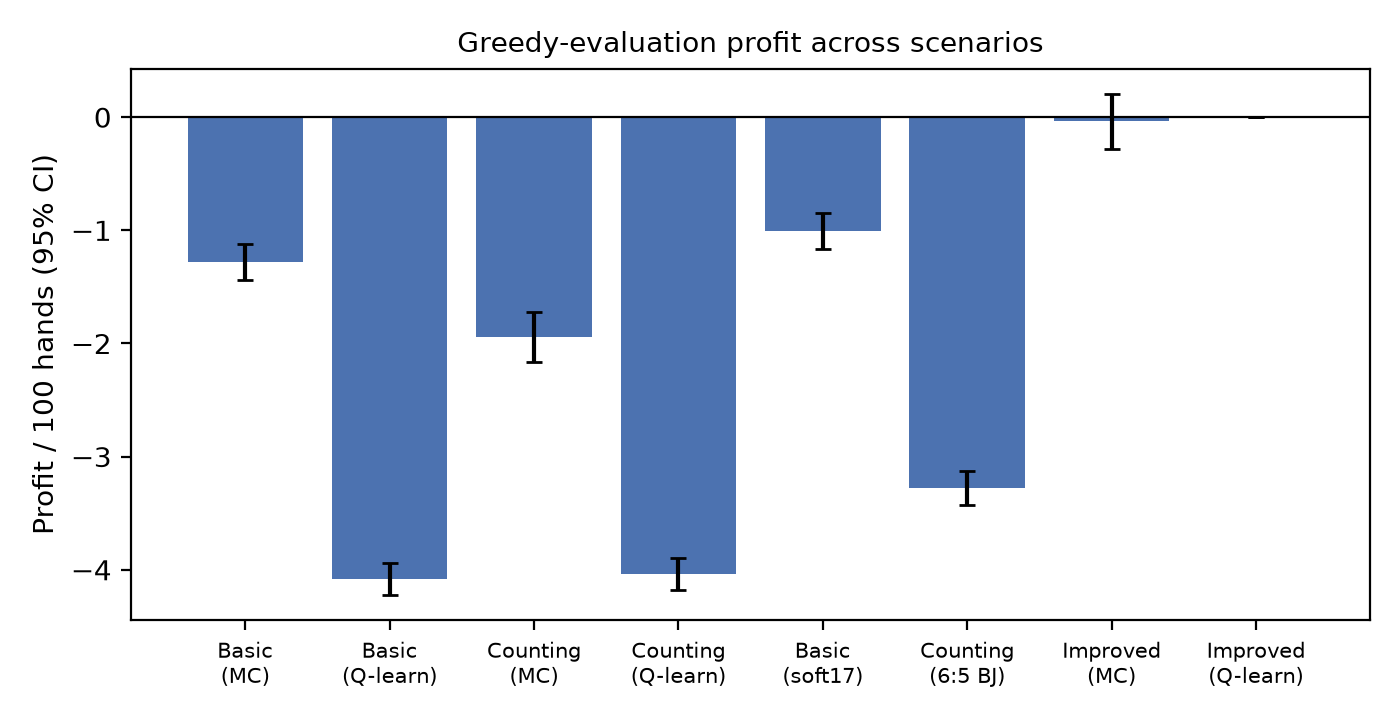
\includegraphics[width=0.98\linewidth]{figs/fig_profit_bars.png}
\caption{Greedy-evaluation profit per 100 hands, all runs (error bars: 95\% CI).}
\label{fig:profit-bars}
\end{figure}

\begin{figure}[t]\centering
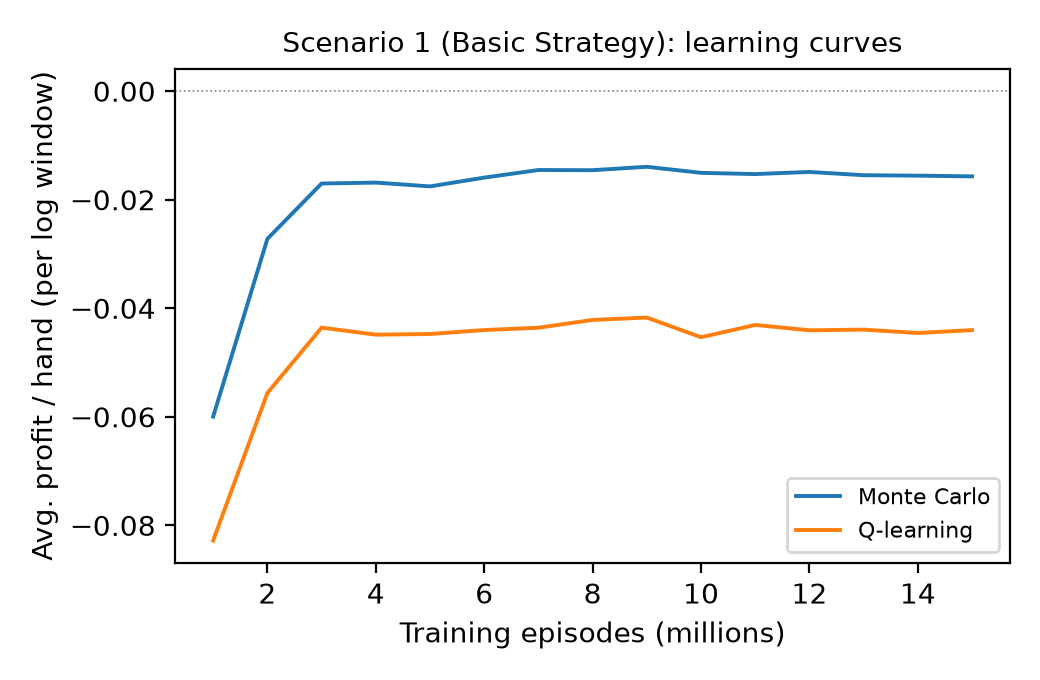
\includegraphics[width=0.98\linewidth]{figs/fig_basic_algo_compare.png}
\caption{Scenario 1 learning curves, Monte Carlo vs.\ Q-learning.}
\label{fig:basic-algo}
\end{figure}

\begin{figure}[t]\centering
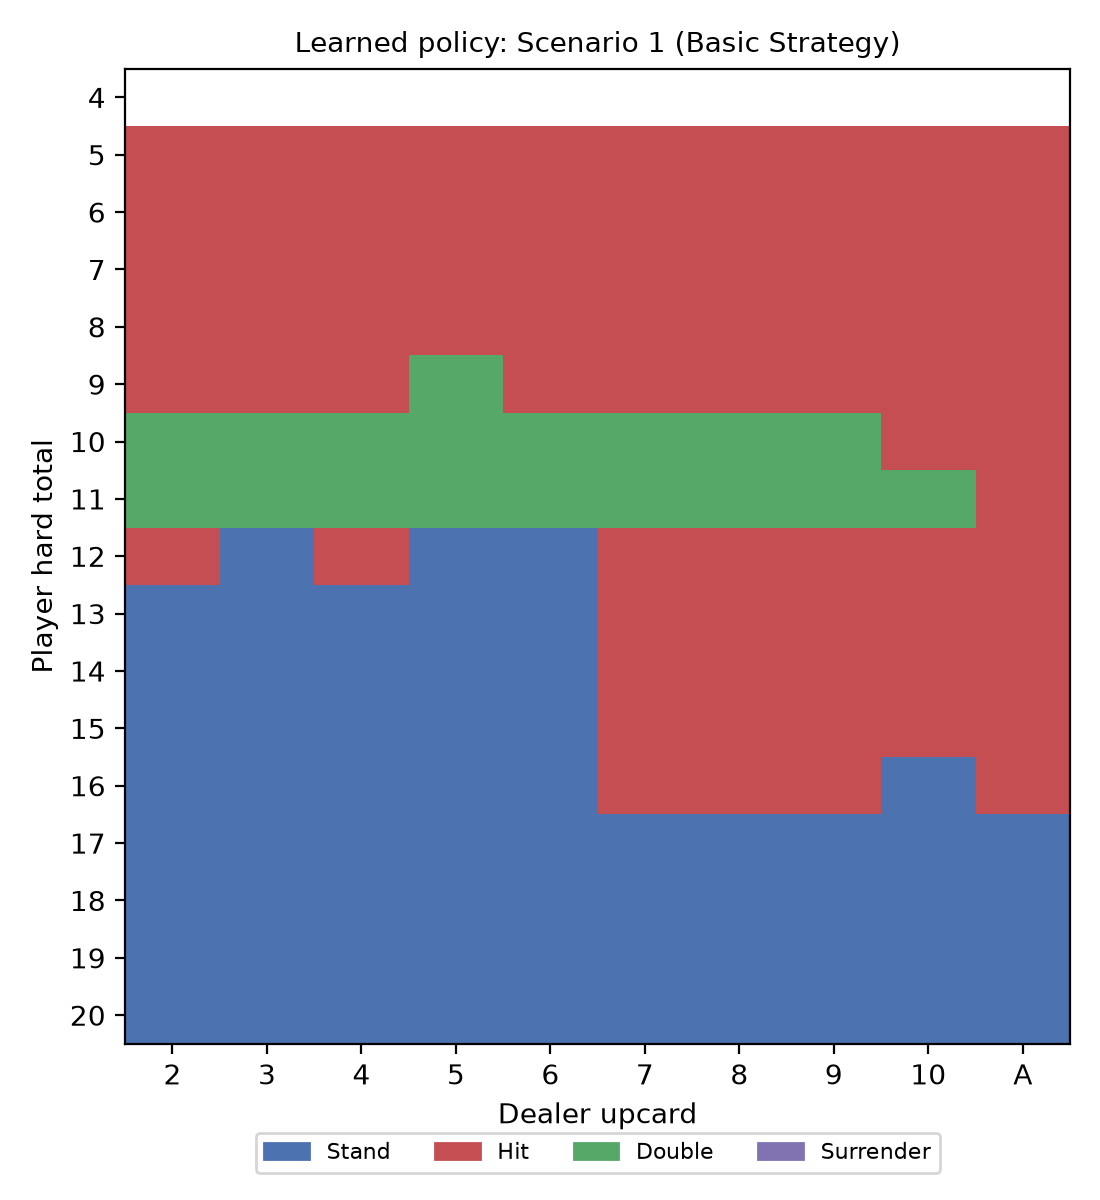
\includegraphics[width=0.98\linewidth]{figs/fig_strategy_heatmap_basic.png}
\caption{Learned Scenario-1 policy on hard totals (Stand/Hit/Double).}
\label{fig:heatmap-basic}
\end{figure}

\section{Conclusion}
\label{sec:conclusion}
We built a Blackjack-playing agent entirely out of tabular reinforcement
learning and plain Python, with no external RL framework, covering basic
strategy, a full Hi-Lo counting system with a learned bet, two rule
variants, and an actual improvement over the counting system rather than
just a restatement of it. Monte Carlo control was the clearly better
algorithm for this task, for reasons tied specifically to how short and
terminal-reward-only Blackjack episodes are, rather than any general claim
about MC versus Q-learning. The betting side of the project is, honestly,
where the more interesting result lives. The first, seemingly reasonable
bandit-based bet-sizing agent quietly failed by converging to never bet at
all. Only inspecting its learned values directly, rather than trusting that
a sensible-looking design must be working, exposed that. Replacing it with
a pooled regression and a Kelly-style bet rule turned a system that refused
to bet into one that closes roughly two-thirds of the gap between the
naive counting strategy and break-even. The main limitation is the one
every tabular method eventually runs into: extending the true count's
resolution, adding more players, or supporting side bets would grow the
state table past what a dictionary can comfortably hold. A natural next
step is a small linear or shallow function approximator over a compact
feature encoding of the same state, which should generalize across the
thinly-visited extreme-count corners identified in Section~\ref{sec:experiments},
instead of needing a dedicated visit count in each one. This would not
require abandoning the ``no external framework'' constraint, since it is
only a modest amount of additional plain Python.

\bibliographystyle{IEEEtran}
\begin{thebibliography}{4}
\bibitem{ieeetemplate} IEEE, ``IEEE Paper Template,'' \url{https://www.ieee.org/conferences/publishing/templates.html}.
\bibitem{suttonbarto} R. S. Sutton and A. G. Barto, \emph{Reinforcement Learning: An Introduction}, 2nd ed. Cambridge, MA: MIT Press, 2018.
\bibitem{thorp} E. O. Thorp, \emph{Beat the Dealer}. New York: Vintage, 1966.
\bibitem{kelly1956} J. L. Kelly Jr., ``A New Interpretation of Information Rate,'' \emph{Bell System Technical Journal}, vol. 35, no. 4, pp. 917--926, 1956.
\end{thebibliography}

\end{document}
